\documentclass{article}


% ------ General Settings ------
\usepackage{graphicx} % 插入图片
\usepackage{hyperref}
\usepackage{amsmath} % 数学符号
\usepackage{booktabs} % 表格样式
\usepackage{geometry}
	\geometry{a4paper,centering,scale=0.8}

% ------ Font Settings ------
\usepackage[UTF8]{ctex}


\renewcommand{\baselinestretch}{1.5}

% ------ Customised Settings ------
\usepackage{ulem}
\newcommand{\tk}{\uline{\hspace{4em}}}

% ------ Environment Settings ------

%% Problem -> https://zhuanlan.zhihu.com/p/472540719
\usepackage{newtxtext}
\usepackage[dvipsnames,svgnames]{xcolor}
\usepackage[strict]{changepage} % 提供一个 adjustwidth 环境
\usepackage{framed} % 实现方框效果

% environment derived from framed.sty: see leftbar environment definition
\definecolor{problemshade}{rgb}{0.95,0.95,1} % 文本背景颜色=242,242,255
\definecolor{problem}{rgb}{0,0,0.478}

\newcounter{prob}
\setcounter{prob}{0}

% 注意行末需要把空格注释掉,不然画出来的方框会有空白竖线
\newenvironment{problem}{%
	\def\FrameCommand{%
		\hspace{1pt}%
		{\color{problem}\vrule width 2pt}%
		{\color{problemshade}\vrule width 4pt}%
		\colorbox{problemshade}%
	}%
	\MakeFramed{\advance\hsize-\width\FrameRestore}%
	\noindent\hspace{-4.55pt}% disable indenting first paragraph
	\begin{adjustwidth}{}{7pt}%
	\vspace{2pt}\vspace{2pt}%
	\refstepcounter{prob}%
	\textbf{Problem \arabic{prob}}%
	\quad%
}%
{%
\vspace{2pt}\end{adjustwidth}\endMakeFramed%
}%


%% Solution
\newenvironment{solution}{
	\par\noindent\textbf{\text{Solution} \quad}
	\citshape
}


%% Hint
\newenvironment{hint}{
	\par\noindent\textbf{\text{Hint} \quad}
	\citshape
}

%% Remark
\newenvironment{remark}{
	\par\noindent\textbf{\text{Remark} \quad}
	\citshape
}

%% Note
\newenvironment{note}{
	\par\noindent\textbf{\text{Note} \quad}
	\citshape
}





















\begin{document}

\begin{center}
	\Large \textbf{欧姆定律小礼物}
\end{center}

\begin{problem}
	司机小王发现他的小车油量表失灵了,打开一看,发现$R'$烧焦了,不知它属于什么型号,再看变阻器$R$的铭牌,上面标有“$50\Omega,1$A”的字样.为了确定被烧焦的电阻$R'$,他拆下车上的油量表,另外找来电源、滑动变阻器$R_1$、定值电阻$R_2$、电压表和开关等器材,用导线连接成如图乙所示的电路进行实验,通过调节滑动变阻器$R_1$的滑片$P$的位置,得到如下表所示的数据(其中$R_2=50\Omega$).已知,如图甲所示的油箱内无油时,$P$在$b$端;油箱装满时,$P$在$a$端.油箱装满油的体积为$60L$,见丙图,油量表是由电流表改装的,它自身的电阻近似为$0$.

    \begin{center}
        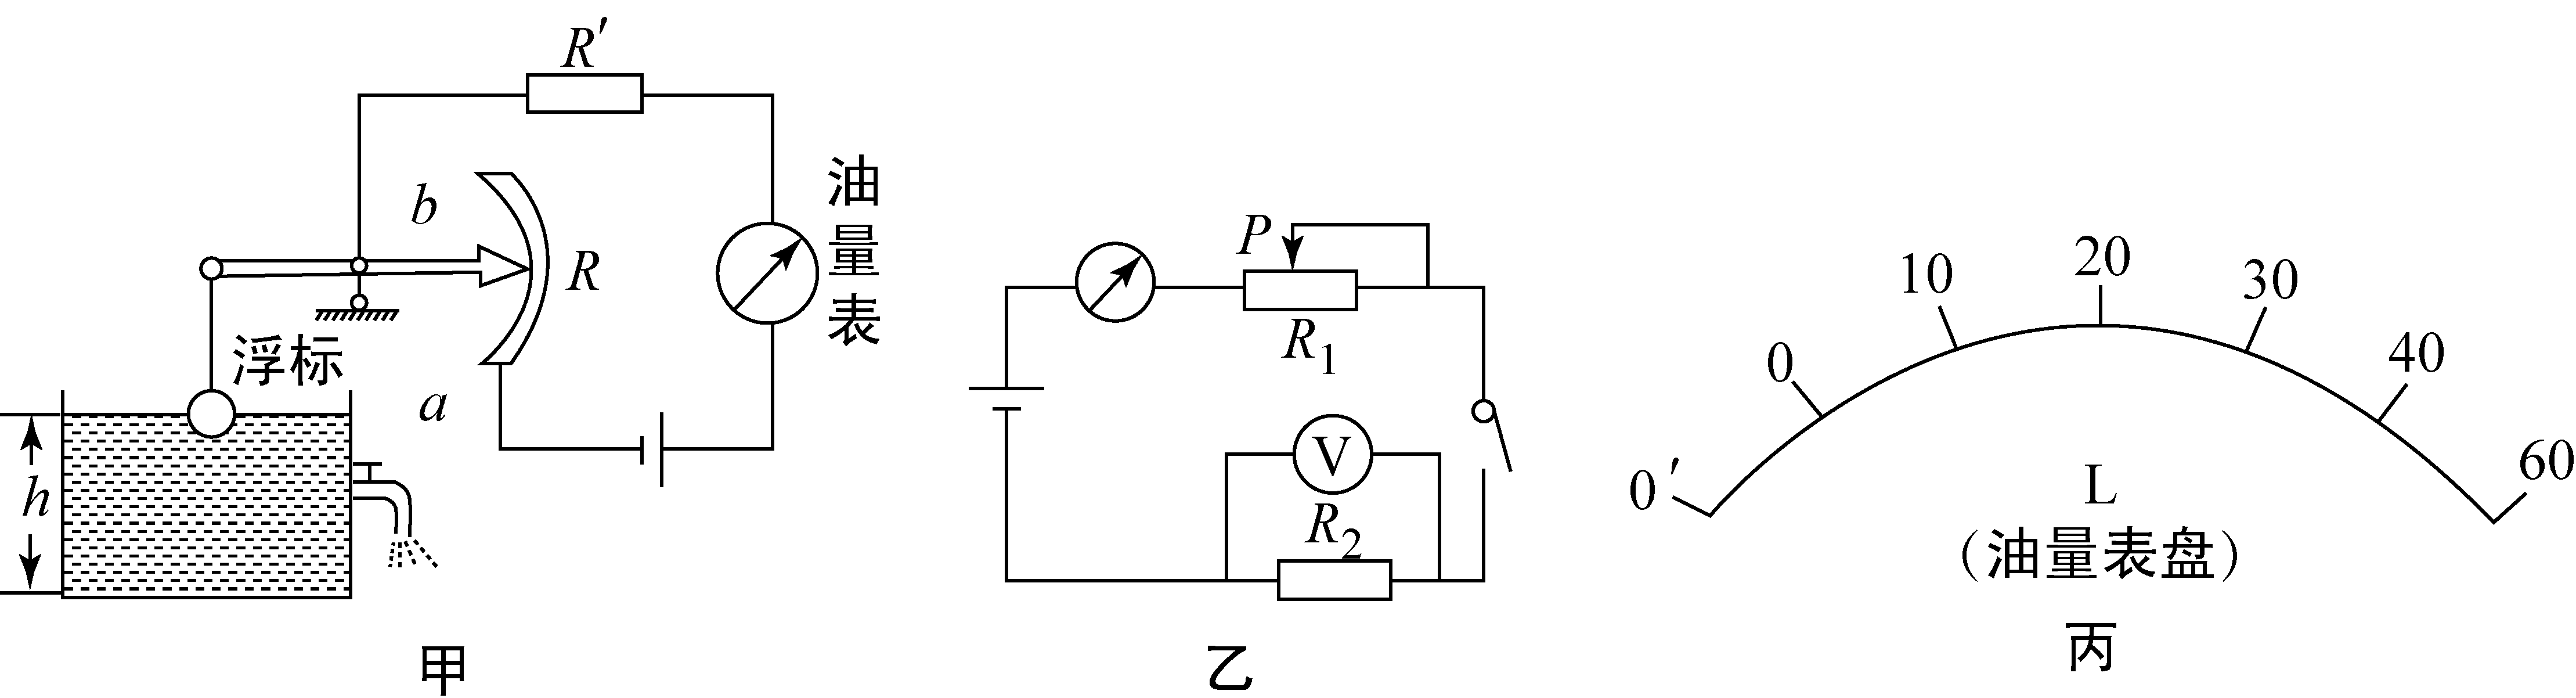
\includegraphics[width=16cm]{attachment/IMG_2174.PNG} 
    \end{center}

    \noindent
    请你帮助司机小王求出:\\
    (1)油量表有最大读数时,通过油量表的电流为\tk A;油量表有最小读数时,通过油量表的电流为\tk A. \\
    (2)图甲中被烧焦的电阻$R'$的阻值为\tk $\Omega$. \\
    (3)在甲图中,当油量表的指针指在刻度盘中央时,滑动变阻器$R$接入的电阻为\tk $\Omega$.
\end{problem}

\begin{hint}
	综合练习
\end{hint}}

\begin{solution}
	请读者自行解答
\end{solution}

\begin{problem}
	如图所示,电源两端电压保持不变,$R_0$为定值电阻.将滑片$P$置于中点,只闭合$S_1$时,电压表的示数为$U$,电流表的示数为$I$.下列情况中电压表和电流表示数变化正确的是

    \begin{center}
        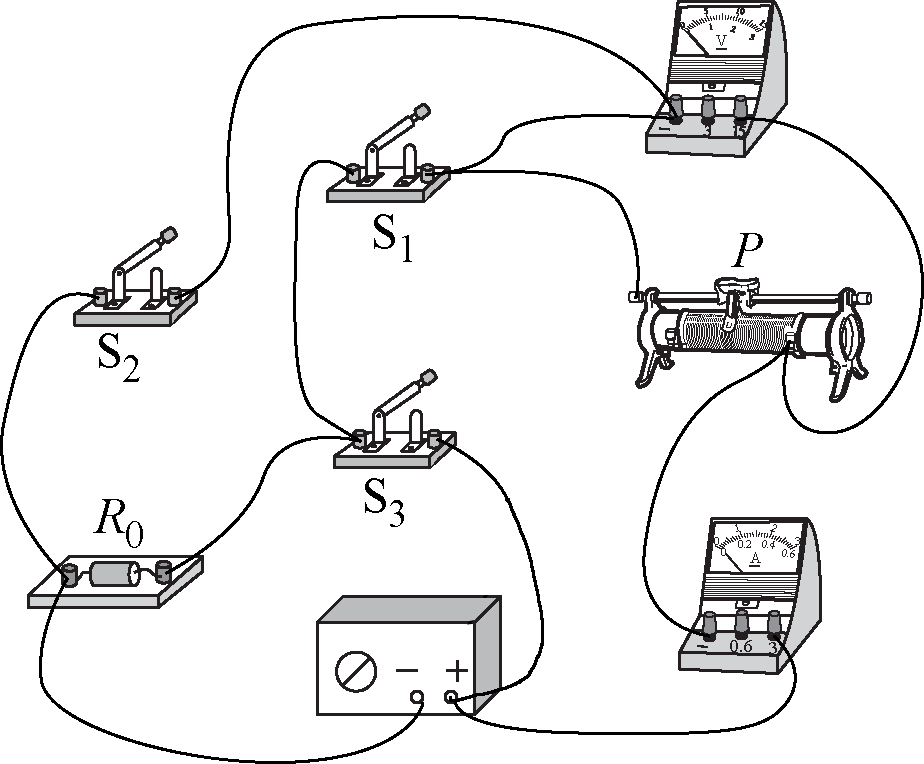
\includegraphics[width=6cm]{attachment/IMG_2215.PNG}
    \end{center}

    \noindent
    A. 断开$S_1$,闭合$S_2$、$S_3$时,滑片$P$向右动,电压表示数不变,电流表示数变大 \\
    B. 断开$S_1$,闭合$S_2$、$S_3$时,滑片$P$向右动,电压表示数变大,电流表示数变大 \\
    C. 只闭合$S_1$,滑片$P$从中点向左移动时,电压表示数变大,电流表示数变小 \\
    D. 只闭合$S_1$,滑片$P$从中点向右移动时,电压表示数不变,电流表示数变大
\end{problem}

\begin{hint}
	动态分析
\end{hint}}

\begin{solution}
	请读者自行解答
\end{solution}

\end{document}